\documentclass[a4paper,11pt,openany]{book}
%\documentclass[a4paper,twoside,11pt,titlepage]{book}
\usepackage{listings}
\usepackage[utf8]{inputenc}
\usepackage[spanish]{babel}

% \usepackage[style=list, number=none]{glossary} %
%\usepackage{titlesec}
%\usepackage{pailatino}

\decimalpoint
\usepackage{dcolumn}
\newcolumntype{.}{D{.}{\esperiod}{-1}}
\makeatletter
\addto\shorthandsspanish{\let\esperiod\es@period@code}
\makeatother


%\usepackage[chapter]{algorithm}
\RequirePackage{verbatim}
%\RequirePackage[Glenn]{fncychap}
\usepackage{fancyhdr}
\usepackage{graphicx}
\usepackage{afterpage}
\usepackage{subfigure}
\usepackage{longtable}

\usepackage[pdfborder={000}]{hyperref} %referencia

% ********************************************************************
% Re-usable information
% ********************************************************************
\newcommand{\myTitle}{Título del proyecto\xspace}
\newcommand{\myDegree}{Grado en ...\xspace}
\newcommand{\myName}{Nombre Apllido1 Apellido2 (alumno)\xspace}
\newcommand{\myProf}{Nombre Apllido1 Apellido2 (tutor1)\xspace}
\newcommand{\myOtherProf}{Nombre Apllido1 Apellido2 (tutor2)\xspace}
%\newcommand{\mySupervisor}{Put name here\xspace}
\newcommand{\myFaculty}{Escuela Técnica Superior de Ingenierías Informática y de
Telecomunicación\xspace}
\newcommand{\myFacultyShort}{E.T.S. de Ingenierías Informática y de
Telecomunicación\xspace}
\newcommand{\myDepartment}{Departamento de ...\xspace}
\newcommand{\myUni}{\protect{Universidad de Granada}\xspace}
\newcommand{\myLocation}{Granada\xspace}
\newcommand{\myTime}{\today\xspace}
\newcommand{\myVersion}{Version 0.1\xspace}


\hypersetup{
pdfauthor = {\myName (email (en) ugr (punto) es)},
pdftitle = {\myTitle},
pdfsubject = {},
pdfkeywords = {palabra_clave1, palabra_clave2, palabra_clave3, ...},
pdfcreator = {LaTeX con el paquete ....},
pdfproducer = {pdflatex}
}

%\hyphenation{}


%\usepackage{doxygen/doxygen}
%\usepackage{pdfpages}
\usepackage{url}
\usepackage{colortbl,longtable}
\usepackage[stable]{footmisc}
%\usepackage{index}

%\makeindex
%\usepackage[style=long, cols=2,border=plain,toc=true,number=none]{glossary}
% \makeglossary

% Definición de comandos que me son tiles:
%\renewcommand{\indexname}{Índice alfabético}
%\renewcommand{\glossaryname}{Glosario}

\pagestyle{fancy}
\fancyhf{}
\fancyhead[LO]{\leftmark}
\fancyhead[RE]{\rightmark}
\fancyhead[RO,LE]{\textbf{\thepage}}
\renewcommand{\chaptermark}[1]{\markboth{\textbf{#1}}{}}
\renewcommand{\sectionmark}[1]{\markright{\textbf{\thesection. #1}}}
\renewcommand\lstlistingname{Listado}

\setlength{\headheight}{1.5\headheight}

\newcommand{\HRule}{\rule{\linewidth}{0.5mm}}


\definecolor{pblue}{rgb}{0.13,0.13,1}
\definecolor{pgreen}{rgb}{0,0.5,0}
\definecolor{pred}{rgb}{0.9,0,0}
\definecolor{pgrey}{rgb}{0.46,0.45,0.48}


\lstset{language=Java,
	showspaces=false,
	showtabs=false,
	breaklines=true,
	showstringspaces=false,
	breakatwhitespace=true,
	commentstyle=\color{pgreen},
	keywordstyle=\color{pblue},
	stringstyle=\color{pred},
	basicstyle=\scriptsize\ttfamily,
	moredelim=[il][\textcolor{pgrey}]{$ $},
	moredelim=[is][\textcolor{pgrey}]{\%\%}{\%\%}
}

\lstset{literate=%
	{á}{{\'a}}1
	{é}{{\'e}}1
	{è}{{\`e}}1
	{í}{{\'i}}1
	{ó}{{\'o}}1
	{ú}{{\'u}}1
	{ñ}{{\~n}}1
}


\newcommand{\bigrule}{\titlerule[0.5mm]}


%Para conseguir que en las páginas en blanco no ponga cabecerass
\makeatletter
\def\clearpage{%
  \ifvmode
    \ifnum \@dbltopnum =\m@ne
      \ifdim \pagetotal <\topskip
        \hbox{}
      \fi
    \fi
  \fi
  \newpage
  \thispagestyle{empty}
  \write\m@ne{}
  \vbox{}
  \penalty -\@Mi
}
\makeatother

\usepackage{pdfpages}
\usepackage{datetime}
\usepackage{geometry,calc}
\usepackage{caption}
\usepackage{csquotes}
\usepackage{algorithm}
\usepackage{algpseudocode}
\usepackage{amsmath}
\usepackage{subfigure}
%%%%%%%%%%%%%%%%%%%%%%%%%%%%%%%%%%%%%%%%%
% Short Sectioned Assignment LaTeX Template Version 1.0 (5/5/12)
% This template has been downloaded from: http://www.LaTeXTemplates.com
% Original author:  Frits Wenneker (http://www.howtotex.com)
% License: CC BY-NC-SA 3.0 (http://creativecommons.org/licenses/by-nc-sa/3.0/)
%%%%%%%%%%%%%%%%%%%%%%%%%%%%%%%%%%%%%%%%%

%----------------------------------------------------------------------------------------
%	PACKAGES AND OTHER DOCUMENT CONFIGURATIONS
%----------------------------------------------------------------------------------------

% ---- Entrada y salida de texto -----

\usepackage[T1]{fontenc} % Use 8-bit encoding that has 256 glyphs
\usepackage[utf8]{inputenc}
%\usepackage{fourier} % Use the Adobe Utopia font for the document - comment this line to return to the LaTeX default

% ---- Idioma --------

\usepackage[spanish, es-tabla]{babel} % Selecciona el español para palabras introducidas automáticamente, p.ej. "septiembre" en la fecha y especifica que se use la palabra Tabla en vez de Cuadro

% ---- Otros paquetes ----

%https://en.wikibooks.org/wiki/LaTeX/Hyperlinks#.5Curl
\usepackage[colorlinks=true,linkcolor=blue,citecolor=red, urlcolor=blue]{hyperref} % para poder poner referencias, url...

%https://en.wikibooks.org/wiki/LaTeX/Colors
\usepackage{color, colortbl}
\usepackage[first=0,last=9]{lcg} %Color tabla
\newcommand{\ra}{\rand0.\arabic{rand}} %Color tabla


\usepackage{eurosym} %Símbolo del euro

\usepackage{amsmath,amsfonts,amsthm} % Math packages
%\usepackage{graphics,graphicx, floatrow} %para incluir imágenes y notas en las imágenes
\usepackage{graphics,graphicx, float, url} %para incluir imágenes y colocarlas

% Para hacer tablas comlejas
%\usepackage{multirow}
%\usepackage{threeparttable}

%\usepackage{sectsty} % Allows customizing section commands
%\allsectionsfont{\centering \normalfont\scshape} % Make all sections centered, the default font and small caps

\usepackage{fancyhdr} % Custom headers and footers
\pagestyle{fancyplain} % Makes all pages in the document conform to the custom headers and footers
\fancyhead{} % No page header - if you want one, create it in the same way as the footers below
\fancyfoot[L]{} % Empty left footer
\fancyfoot[C]{} % Empty center footer
\fancyfoot[R]{\thepage} % Page numbering for right footer
\renewcommand{\headrulewidth}{0pt} % Remove header underlines
\renewcommand{\footrulewidth}{0pt} % Remove footer underlines
\setlength{\headheight}{13.6pt} % Customize the height of the header
\usepackage{pdfpages}
\numberwithin{equation}{section} % Number equations within sections (i.e. 1.1, 1.2, 2.1, 2.2 instead of 1, 2, 3, 4)
\numberwithin{figure}{section} % Number figures within sections (i.e. 1.1, 1.2, 2.1, 2.2 instead of 1, 2, 3, 4)
\numberwithin{table}{section} % Number tables within sections (i.e. 1.1, 1.2, 2.1, 2.2 instead of 1, 2, 3, 4)

\setlength\parindent{0pt} % Removes all indentation from paragraphs - comment this line for an assignment with lots of text

\newcommand{\horrule}[1]{\rule{\linewidth}{#1}} % Create horizontal rule command with 1 argument of height

\begin{document}
\begin{titlepage}
\newlength{\centeroffset}
\setlength{\centeroffset}{-0.5\oddsidemargin}
\addtolength{\centeroffset}{0.5\evensidemargin}
\thispagestyle{empty}

\noindent\hspace*{\centeroffset}\begin{minipage}{\textwidth}

\centering

\includegraphics[width=0.9\textwidth]{imagenes/logo_ugr.jpg}\\[1.4cm]

\textsc{ \Large PRÁCTICA PROCESOS GAUSSIANOS\\[0.2cm]}
\textsc{ Máster DATCOM }\\[1cm]
% Upper part of the page
% 
% Title
{\Huge\bfseries Extracción de Características en Imágenes\\
}
\noindent\rule[-1ex]{\textwidth}{3pt}\\[3.5ex]
{\large\bfseries }
\end{minipage}

\vspace{1cm}
\noindent\hspace*{\centeroffset}\begin{minipage}{\textwidth}
\centering

\textbf{Autor}\\ {Alberto Armijo Ruiz}\\[2.5ex]

\includegraphics[width=0.3\textwidth]{imagenes/etsiit_logo.png}\\[0.1cm]
\textsc{Escuela Técnica Superior de Ingenierías Informática y de Telecomunicación}\\
\textsc{---}\\
\today
\end{minipage}
%\addtolength{\textwidth}{\centeroffset}
%\vspace{\stretch{2}}
\end{titlepage}
%\chapter*{}
\section{Resumen}
En esta práctica se realizará un estudio sobre diferentes tipos de descriptores de imágenes; en concreto HOG (Histogram of Gradients) y LBP (Local Binary Patterns). De este último se realizará una modificación, para cuál también se realizará un estudio con diferentes clasificadores. Por último, se describirá el proceso para crear un detector de personas en imágenes con uno de los clasificadores generados en los apartados anteriores y se analizarán los resultados que produce. \\

Esta práctica ha sido realizada en Python 3 junto con OpenCV. Dentro del fichero comprimido se encontrarán los diferentes archivos con la implementación de los descriptores, los archivos de pruebas, el archivo con los resultados, y el archivo que contiene la implementación del detector de personas. Adicionalmente se proporcionan archivos con los datos generados por los descriptores comprimidos ya que tardan bastante en cargarse de forma normal por si se desea ejecutar las pruebas con los diferentes descriptores.

%\frontmatter
\tableofcontents
\listoffigures
\listoftables
%
%\mainmatter
%\setlength{\parskip}{5pt}
\chapter{Parte Práctica}
\section{Ejercicio 1}
En este ejercicio se debe entrenar un modelo \textit{HoeffdingTree} con un flujo de datos generado con \textit{WaveformGenerator}, semilla inicializada a 2 y un millón de instancias. Tras esto se debe utilizar otro flujo generado con \textit{WaveformGenerator} utilizando como semilla el 4 y un millón de datos. Tras esto se debe probar el modelo \textit{HoeffdingAdaptiveTree} con los mismo paramétros. Dado que con un solo ejemplo no vale para saber que algoritmo es mejor que otro, se realizarán 10 pruebas con cada uno de los clasificadores y se estudiaran los resultados obtenidos.

Las sentencias necesarias para realizar lo anterior son las siguientes:
\vspace{0.06in}

\textit{java -cp moa.jar moa.DoTask ``EvaluateModel -m
(LearnModel -l trees.HoeffdingTree -s
(generators.WaveformGenerator -i 2) -m 1000000)
-s (generators.WaveformGenerator -i 4)``}

\textit{java -cp moa.jar moa.DoTask ``EvaluateModel -m
(LearnModel -l trees.HoeffdingAdaptiveTree -s
(generators.WaveformGenerator -i 2) -m 1000000)
-s (generators.WaveformGenerator -i 4)``}
\vspace{0.06in}


Las opciones que se pueden ver en las sentencias son las siguientes:
\begin{itemize}
	\item \textit{EvaluateModel} -m: para expecificar el modelo.
	\item \textit{LearnModel} -l: para expecificar modelo que se va a entrenar.
	\item \textit{LearnModel} -s: para el flujo de datos con el que se entrena el modelo.
	\item \textit{LearnModel} -m: para expecificar el número de instancias con el que se entrena el modelo.
	\item \textit{WaveformGenerator} -i: para expecificar la semilla con la que se inicializa el generador.
	\item \textit{EvaluateModel} -s: para expecificar el flujo de datos con el que se evalúa el modelo que ha sido entrenado.
\end{itemize}

Para realizar las pruebas con diferentes semillas se han creados dos scripts para automatizar el proceso. Tras esto se han mirado los resultados y se ha realizado un test para ver si existen diferencias entre ambos algoritmos.

\begin{figure}[H]
	\centering
	\subfigure[script para HoeffdingTree]{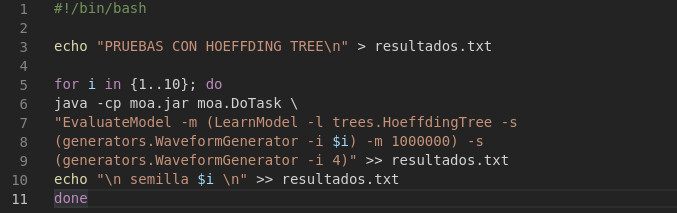
\includegraphics[width=80mm]{imagenes/script_hoeff}}
	\subfigure[script para HoeffdingAdaptiveTree]{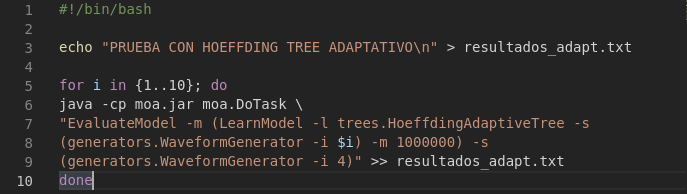
\includegraphics[width=80mm]{imagenes/script_hoeff_adapt}}
	\caption{Scripts para generar las pruebas de forma automática}
	\label{fig:scripts1}
\end{figure}

Los resultados obtenidos por los clasificadores son los siguientes.
\begin{table}[H]
	\begin{tabular}{lllll}
		\textbf{Semilla} & \textbf{Accuracy} & \textbf{Kappa} & \textbf{Accuracy Adaptive} & \textbf{Kappa Adaptive} \\ \hline
		1                & 84,509            & 76,765         & 84,521                     & 76,783                  \\
		2                & 84,512            & 76,77          & 84,474                     & 76,712                  \\
		3                & 84,59             & 76,887         & 84,416                     & 76,625                  \\
		4                & 84,666            & 77,001         & 84,465                     & 76,699                  \\
		5                & 84,481            & 76,723         & 84,262                     & 76,395                  \\
		6                & 84,342            & 76,514         & 84,368                     & 76,554                  \\
		7                & 84,799            & 77,2           & 84,271                     & 76,408                  \\
		8                & 84,153            & 76,231         & 84,243                     & 76,36                   \\
		9                & 84,641            & 76,963         & 84,478                     & 76,719                  \\
		10               & 84,578            & 76,869         & 84,326                     & 76,491                 
	\end{tabular}
\label{table:1}
\caption{Resultados pruebas ejercicio 1}
\end{table}

Como se puede ver los valores son muy similares, aún así se utilizará un test para confirmar que no hay diferencias de rendimiento entre ambos clasificadores.

\begin{figure}[H]
	\centering
	\subfigure[test de normalidad]{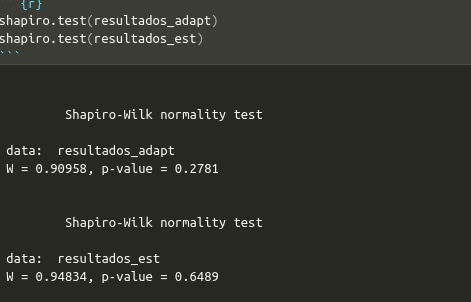
\includegraphics[width=40mm]{imagenes/normality_ej1}}
	\subfigure[test de wilcoxon]{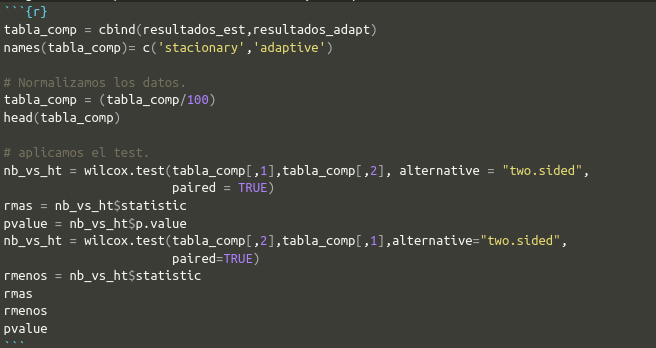
\includegraphics[width=65mm]{imagenes/wilc_ej1}	}
\end{figure}

El resultado del test de Wilcoxon es: 0.03710938

Por lo que se puede ver en los resultados, los dos algoritmos están ofreciendo los mismos resultados; esto puede ser posiblemente porque estamos entrenando ambos algoritmos de forma offline, por lo cual tanto HoeffdingTree como HoeffdingAdaptiveTree están aprendiendo sobre el mismo conjunto de datos y no son capaces de responder a cambios de concepto como el que tiene el flujo de datos generado con la semilla 4. Además, si realizamos un estudio sobre los resultados, el test muestra que existen diferencias significativas entre ambos algoritmos, pero después la diferencia entre la mediana de un algoritmo y otro son casi inexistentes.

\section{Ejercicio 2}
Para este ejercicio se debe hacer lo mismo que en el anterior pero cambiando el método de evaluación por \textit{InterleavedTestThenTrain}. A diferencia que en el ejercicio anterior, no se necesita entrenar un modelo, ya que el método de evaluación \textit{InterleavedTestThenTrain} primero testea los datos y después los utiliza para entrenar, por lo tanto está entrenando y testeando datos durante todo el proceso.Las sentencias necesarias para evaluar los modelos son los siguientes:
\vspace{0.06in}

\textit{java -cp moa.jar moa.DoTask \\
``EvaluateInterleavedTestThenTrain -l
trees.HoeffdingTree -s
(generators.WaveformGenerator -i 2)
-i 1000000 -f 10000`` > resultados\_online.txt}

\textit{java -cp moa.jar moa.DoTask \\
``EvaluateInterleavedTestThenTrain -l
trees.HoeffdingAdaptiveTree -s
(generators.WaveformGenerator -i 2)
-i 1000000 -f 10000`` > resultados\_online\_adative.txt}

Las opciones que se muestran para estas sentencias son las mismas que para el ejercicio anterior menos la opción -l de \textit{EvaluateInterleavedTestThenTrain}; esta función se utiliza  para evaluar un modelo con Test-Then-Train especificado mediante la opción -l. Las otras opciones que se pueden ver son -i que especifica el número de instancias totales con las que se evaluará el modelo y -f que especifica el número de instancias que llegan en cada momento.

Para realizar un estudio sobre ambos modelos; \textit{HoeffdingTree} y \textit{HoeffdingAdaptiveTree}, se han creado dos scripts para realizar pruebas con diferentes valores para la semilla de inicialización del generador \textit{WavefromGenerator}. Los scripts son los siguientes:

\begin{figure}[H]
	\centering
	\subfigure[script para HoeffdingTree]{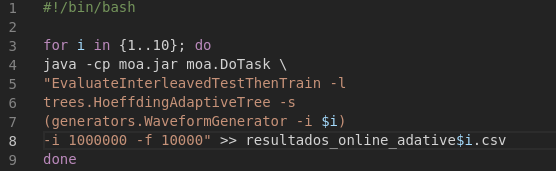
\includegraphics[width=80mm]{imagenes/script_online_hoeff}}
	\subfigure[script para HoeffdingAdaptiveTree]{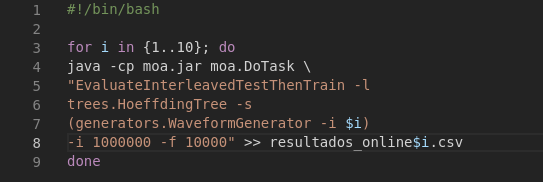
\includegraphics[width=80mm]{imagenes/script_online_adapt}}
	\caption{Scripts para generar las pruebas de forma automática con EvaluateInterleavedTestThenTrain}
	\label{fig:scripts2}
\end{figure}

Los resultados obtenidos por los clasificadores son los siguientes.
\begin{table}[H]
	\begin{tabular}{lllll}
		\textbf{Semilla} & \textbf{Accuracy} & \textbf{Accuracy Adaptive} & \textbf{Kappa} & \textbf{Kappa Adaptive} \\ \hline
		1                & 83,8903           & 83,8042                    & 75,83623569    & 75,7071683              \\
		2                & 83,7851           & 83,7313                    & 75,67749802    & 75,5967623              \\
		3                & 83,8876           & 83,7875                    & 75,82954147    & 75,6792025              \\
		4                & 84,0451           & 83,7961                    & 76,06946036    & 75,69604195             \\
		5                & 83,8402           & 83,7144                    & 75,75999473    & 75,57128698             \\
		6                & 83,9062           & 83,8406                    & 75,85905507    & 75,76071273             \\
		7                & 83,8867           & 83,7784                    & 75,82927699    & 75,66688337             \\
		8                & 83,8687           & 83,8968                    & 75,8028419     & 75,84506754             \\
		9                & 83,7875           & 83,8282                    & 75,6817212     & 75,7427829              \\
		10               & 83,8479           & 83,9                       & 75,77149369    & 75,84955066            
	\end{tabular}
\label{table:2}
\caption{Resultados pruebas ejercicio 2}
\end{table}

Al igual que en el ejercicio anterior, no parece haber diferencias entre los dos algoritmos; aún así se realizará un test para ver si existen diferencias entre ellos.


Para ver si hay diferencias significativas entre ambos algoritmos, cargaremos los datos y comprobaremos si existen diferencias significativas.La forma de comprobar la normalidad de las soluciones y el test se realiza de la misma forma que en el ejercicio anterior. Al igual que en el ejercicio anterior, los resultados nos siguen una distribución normal, por lo que se utilizará el test de Wilcoxon para comprobar si hay diferencias de rendimiento entre ambos algoritmos.

Por los resultados del test (0.02734375), debería de haber diferencias significativas, pero al hacer la media de la precisión de ambos algoritmos se puede ver que son casi iguales, por lo que descartaremos la hipótesis del test y diremos que no hay diferencias entre los algoritmos. Es normal que no haya diferencias significativas entre los modelos, ya que a no ser que en el flujo de datos haya un cambio de concepto ambos modelos se comportan de forma igual.

\section{Ejercicio 3}
Para este ejercicio se debe entrenar un \textit{HoeffdingTree} online con test-then-train sobre 2M de instancias y freq. muestreo de 100k generando los datos con un generador \textit{RandomRBFGeneratorDrift}, con semilla aleatoria igual a 1 para generación de instancias, generando 2 clases, 7 atributos, 3 centroides, drift en todos los centroides y velocidad de cambio igual a 0.001. También se probará el modelo \textit{HoeffdingAdaptiveTree}. Las sentencias necesarias para ejecutar ambos modelos son las siguientes:
\vspace{0.06in}

\textit{java -cp moa.jar moa.DoTask \\``EvaluateInterleavedTestThenTrain -l trees.HoeffdingTree -s\\
(generators.RandomRBFGeneratorDrift -s 0.001 -k 3 -r 1 -i 1 -a 7 -n 3)
-i 2000000 -f 100000``
}

\textit{java -cp moa.jar moa.DoTask \\``EvaluateInterleavedTestThenTrain -l trees.HoeffdingAdaptiveTree -s\\
(generators.RandomRBFGeneratorDrift -s 0.001 -k 3 -r 1 -i 1 -a 7 -n 3)
-i 2000000 -f 100000``}

\vspace{0.06in}

Las nuevas opciones que hay a diferencia de los ejercicios anteriores son las opciones del generador \textit{RandomRBFGeneratorDrift}. La opción -s especifica la velocidad de cambio en los centroides, la opción -r especifica la semilla para la generación de modelos, la opción -i especifica la semilla para la generación de instancias, la opción -a especifica el número de atributos que tiene cada instancia, la opción -k especifica el número de centroides que cambian y la opción -n especifica el número de centroides del flujo de datos.
\newline

Para realizar un estudio sobre el comportamiento de los algoritmos, se ha utilizado la GUI de MOA para poder ver una gráfica sobre la precisión de los modelos sobre el flujo de datos que se genera. Para este ejercicio se han utilizado 3 semillas diferentes para cada uno de los modelos, los resultados obtenidos son los siguientes.

\begin{figure}[H]
	\centering
	\subfigure[HoeffdingTree]{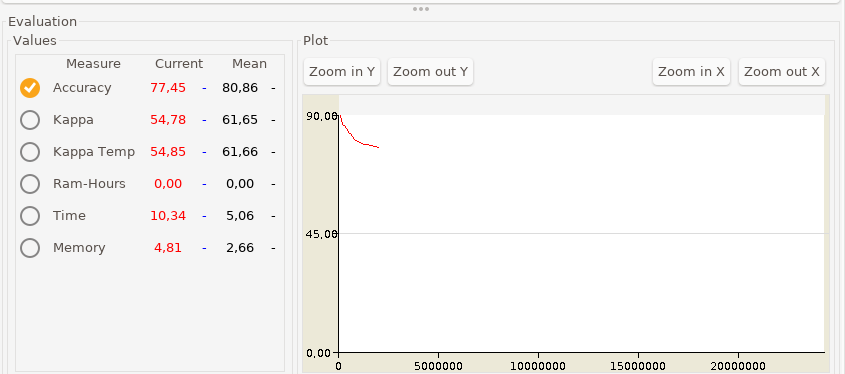
\includegraphics[width=70mm]{imagenes/rbf_drift_s1}}
	\subfigure[HoeffdingAdaptiveTree]{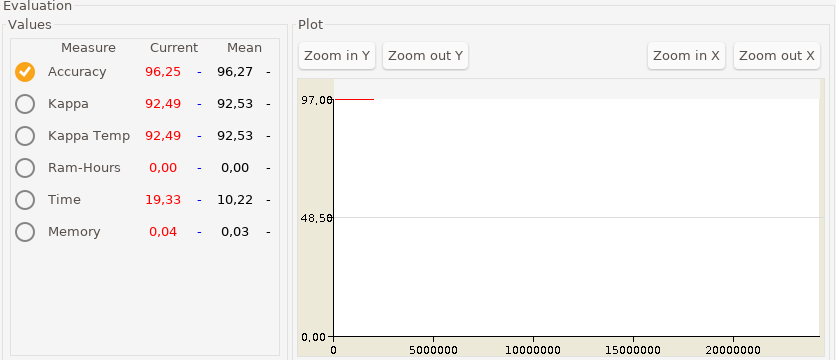
\includegraphics[width=70mm]{imagenes/rbf_drift_s1_adapt}}
	\caption{Resultados InterleavedTestThenTrain con semilla 1}
	\label{fig:res31}
\end{figure}

\begin{figure}[H]
	\centering
	\subfigure[HoeffdingTree]{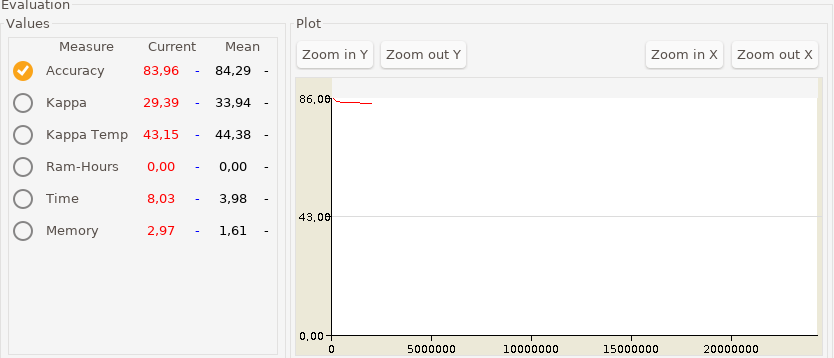
\includegraphics[width=70mm]{imagenes/rbf_drift_s2}}
	\subfigure[HoeffdingAdaptiveTree]{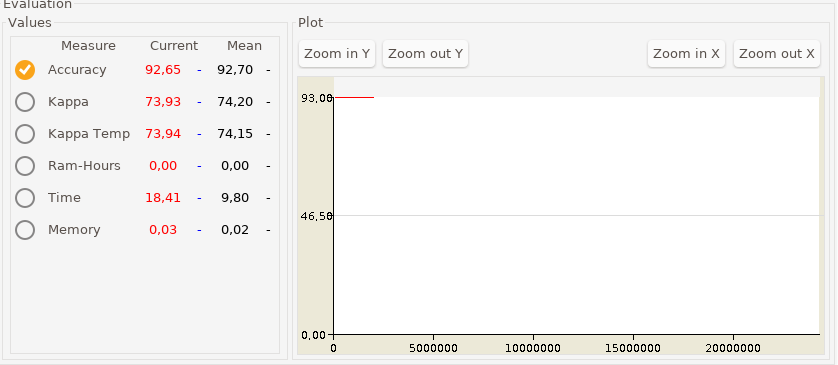
\includegraphics[width=70mm]{imagenes/rbf_drift_s2_adapt}}
	\caption{Resultados InterleavedTestThenTrain con semilla 2}
	\label{fig:res32}
\end{figure}

\begin{figure}[H]
	\centering
	\subfigure[HoeffdingTree]{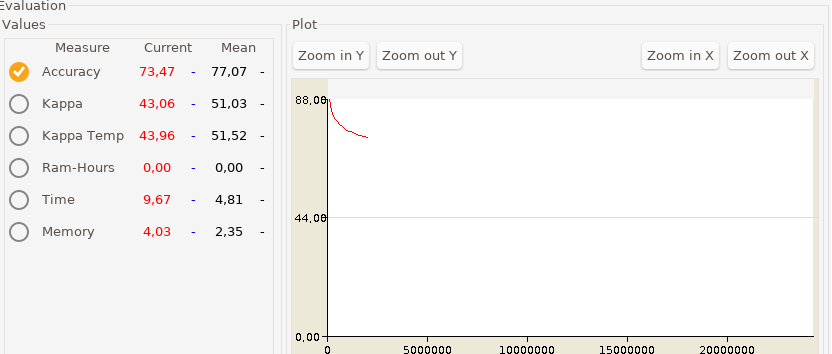
\includegraphics[width=70mm]{imagenes/rbf_drift_s3}}
	\subfigure[HoeffdingAdaptiveTree]{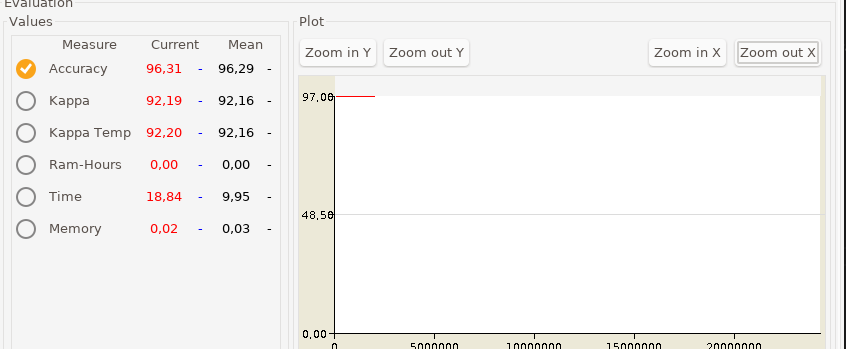
\includegraphics[width=70mm]{imagenes/rbf_drift_s3_adapt}}
	\caption{Resultados InterleavedTestThenTrain con semilla 3}
	\label{fig:res33}
\end{figure}
Si nos fijamos en los resultados que se pueden ver en las imágenes
de la GUI de MOA, se puede ver que el clasificador \textit{HoeffdingTree} obtiene
peores resultados que su versión adaptativa, esto es así porque el
algoritmo \textit{HoeffdingTree} no está preparado para los cambios de concepto,
por ello cuando hay un cambio de concepto la precisión del algoritmo
baja bastante. En cambio, el clasificador \textit{HoeffdingAdaptiveTree} sí que
está preparado para detectar cambios de concepto, para ello utiliza el
método \textit{ADWIN}, una vez detectado el cambio de concepto puede re-entrenar
el árbol, podar ciertas ramas que ya no sirvan, etc. Por ello, no
sufre una bajada en la precisión como le pasa al algoritmo \textit{HoeffdingTree}
y es apto para clasificación con flujos que tienen cambios de concepto.

\section{Ejercicio 4}
Igual que el modelo anterior, pero utilizando la función Prequential en vez de la función TestThenTrain. El método de evaluación Prequential testea con cada ejemplo que se le va entrando y después reentrena el modelo; utiliza una ventana para ir olvidando ejemplos antiguos y centrarse en ejemplos nuevos. La sentencias necesarias para evaluar es la siguiente.
\vspace{0.06in}

\textit{java -cp moa.jar moa.DoTask \\ ``EvaluatePrequential -l trees.HoeffdingTree
-e (WindowClassificationPerformanceEvaluator -w 1000) -s
(generators.RandomRBFGeneratorDrift -s 0.001 -k 3 -r 1 -i 1 -a 7 -n 3)
-i 2000000``}

\textit{java -cp moa.jar moa.DoTask \\ ``EvaluatePrequential -l trees.HoeffdingAdaptiveTree
-e (WindowClassificationPerformanceEvaluator -w 1000) -s
(generators.RandomRBFGeneratorDrift -s 0.001 -k 3 -r 1 -i 1 -a 7 -n 3)
-i 2000000``}

Al igual que en el ejercicio anterior, se han hecho pruebas con 3 semillas diferentes. Los resultados son los siguientes.

\begin{figure}[H]
	\centering
	\subfigure[HoeffdingTree]{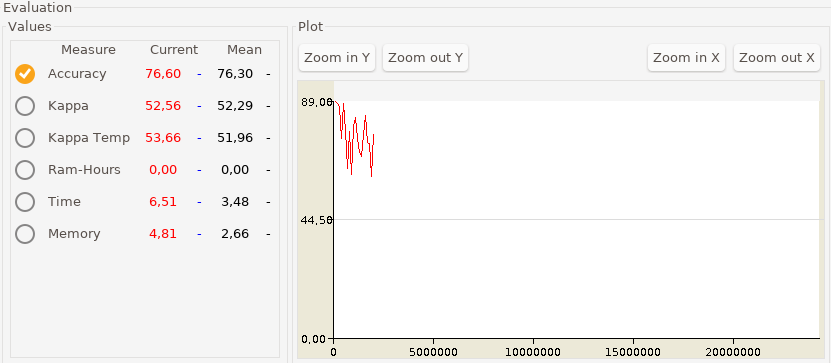
\includegraphics[width=70mm]{imagenes/prequential_s1}}
	\subfigure[HoeffdingAdaptiveTree]{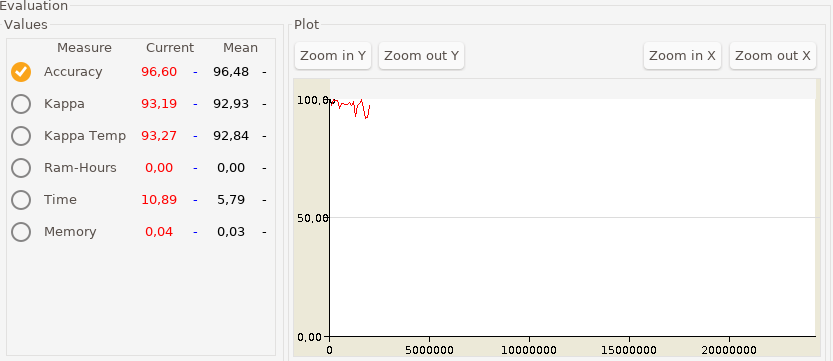
\includegraphics[width=70mm]{imagenes/prequential_adaptive_s1}}
	\caption{Resultados Prequential con semilla 1}
	\label{fig:res41}
\end{figure}

\begin{figure}[H]
	\centering
	\subfigure[HoeffdingTree]{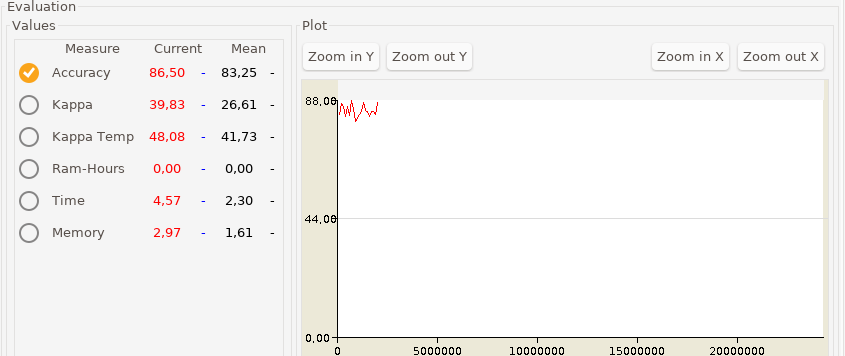
\includegraphics[width=70mm]{imagenes/prequential_s2}}
	\subfigure[HoeffdingAdaptiveTree]{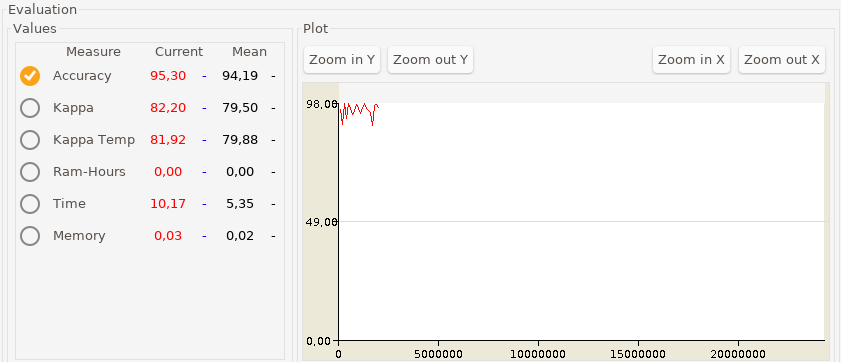
\includegraphics[width=70mm]{imagenes/prequential_adaptive_s2}}
	\caption{Resultados Prequential con semilla 2}
	\label{fig:res42}
\end{figure}

\begin{figure}[H]
	\centering
	\subfigure[HoeffdingTree]{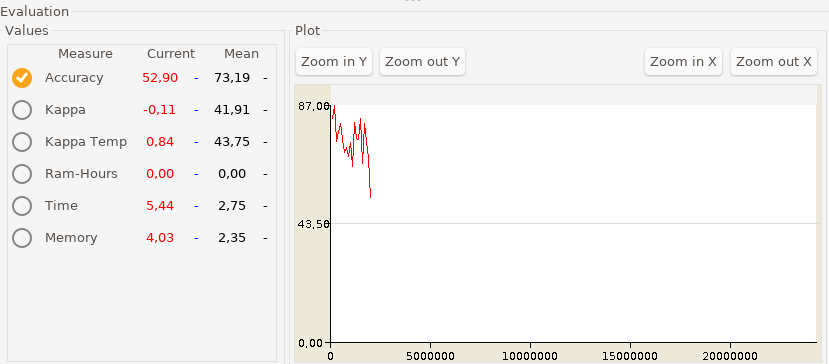
\includegraphics[width=70mm]{imagenes/prequential_s3}}
	\subfigure[HoeffdingAdaptiveTree]{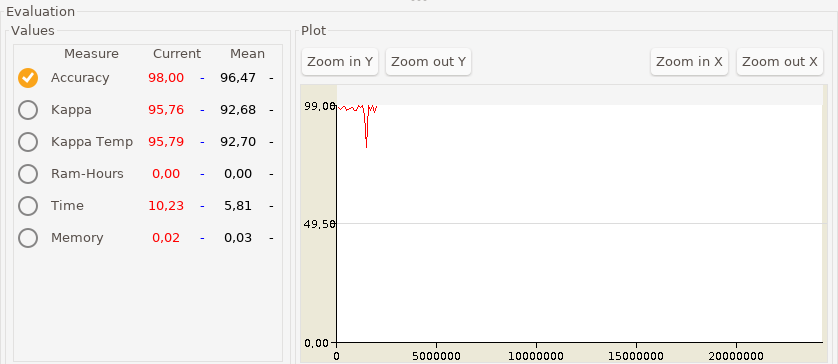
\includegraphics[width=70mm]{imagenes/prequential_adaptive_s3}}
	\caption{Resultados Prequential con semilla 3}
	\label{fig:res43}
\end{figure}
\vspace{0.06in}

Realizando pruebas con ambos algoritmos, se puede ver una gran diferencia
entre cada uno de los algoritmos. El clasificador \textit{HoeffdingTree} sufre una
gran bajada en la precisión cuando llega un cambio de concepto, y para
cuando puede recuperarse vuelve a haber otro cambio de concepto; por lo
que su rendimiento vuelve a bajar. Por otro lado, el clasificador
\textit{HoeffdingAdaptiveTree} al detectar los cambios de concepto, tiene pequeñas
bajadas en la precisión de las cuales se recupera rápidamente. Por lo tanto
para este tipo de flujo de datos el clasificador \textit{HoeffdingAdaptiveTree}
es mejor que \textit{HoeffdingTree}.

\section{Ejercicio 5}
Repetir el ejercicio anterior cambiando el modelo con \textit{SingleClassfierDrift},
utilizando el modelo \textit{HoeffdingTree}. Este método, reemplaza el clasificador
cuando se detecta un cambio de concepto. La sentencia necesaria para ejecutar
la evaluación del modelo es la siguiente:

\textit{java -cp moa.jar moa.DoTask \\ ``EvaluateInterleavedTestThenTrain -l
(drift.SingleClassifierDrift -l trees.HoeffdingTree) -s
(generators.RandomRBFGeneratorDrift -s 0.001 -k 3 -r 1 -i 1 -a 7 -n 3)
-i 2000000 -f 100000``}

Para la modificación con el modelo HoeffdingAdaptiveTree habría que utilizar
la siguiente sentencia:
\textit{java -cp moa.jar moa.DoTask \\ ``EvaluateInterleavedTestThenTrain -l
(drift.SingleClassifierDrift -l trees.HoeffdingAdaptiveTree) -s
(generators.RandomRBFGeneratorDrift -s 0.001 -k 3 -r 3 -i 3 -a 7 -n 3)
-i 2000000 -f 100000``}

La única opción nueva con respecto al resto de ejercicios es la opción -l de la acción \textit{SingleClassifierDrift} que especifica que modelo tiene que utilizar este método.

Al igual que en el ejercicio 3, se han ejecutado los algoritmos con tres semillas diferentes para el generador \textit{RandomRBFGeneratorDrift}. Los resultados obtenidos por los clasificadores son los siguientes.

\begin{figure}[H]
	\centering
	\subfigure[HoeffdingTree]{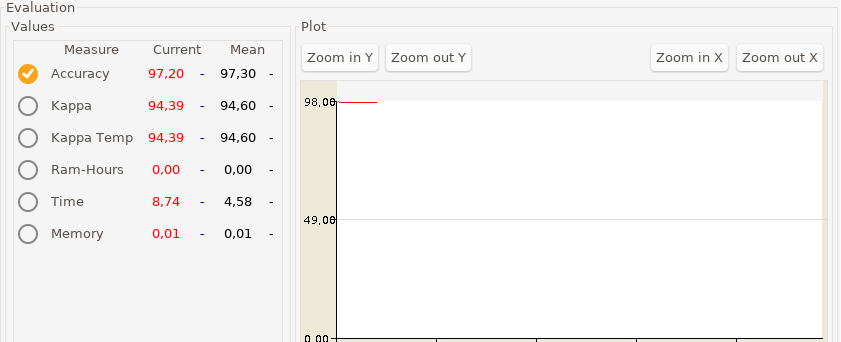
\includegraphics[width=70mm]{imagenes/singledrift_hoff}}
	\subfigure[HoeffdingAdaptiveTree]{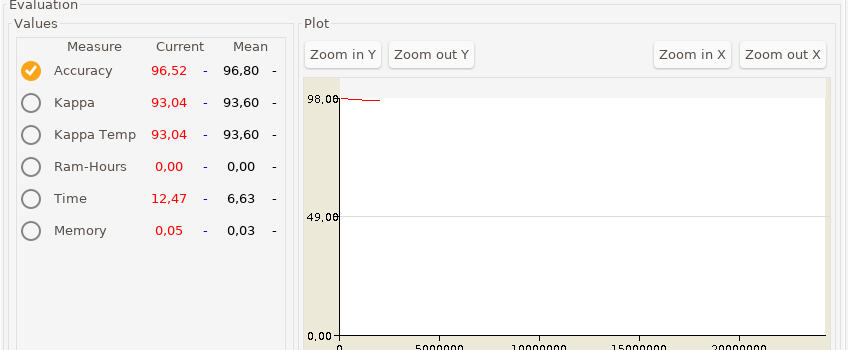
\includegraphics[width=70mm]{imagenes/singledrift_hoffadp}}
	\caption{Resultados SingleClassifierDrift con semilla 1}
	\label{fig:res51}
\end{figure}

\begin{figure}[H]
	\centering
	\subfigure[HoeffdingTree]{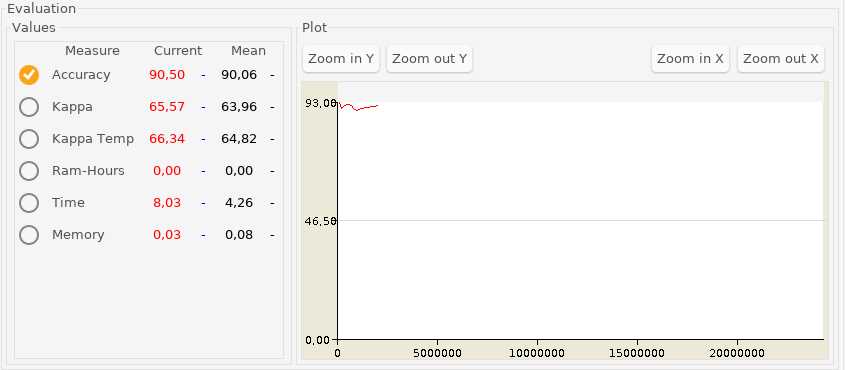
\includegraphics[width=70mm]{imagenes/singledrift_hoffs2}}
	\subfigure[HoeffdingAdaptiveTree]{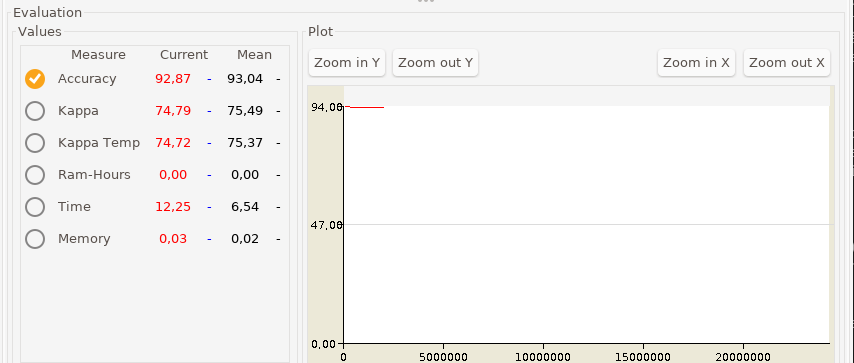
\includegraphics[width=70mm]{imagenes/singledrift_hoffadps2}}
	\caption{Resultados SingleClassifierDrift con semilla 2}
	\label{fig:res52}
\end{figure}

\begin{figure}[H]
	\centering
	\subfigure[HoeffdingTree]{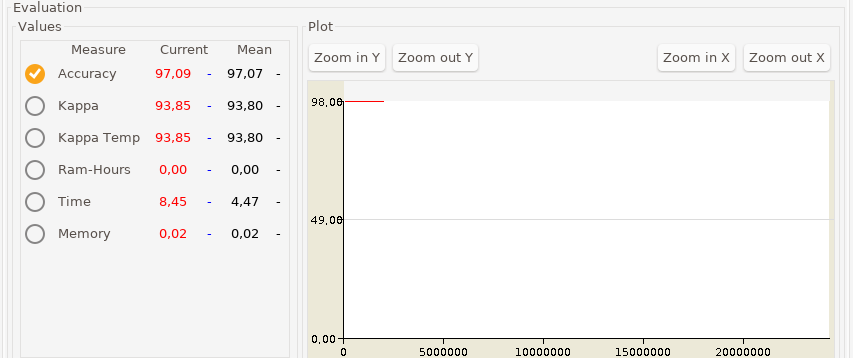
\includegraphics[width=70mm]{imagenes/singledrift_hoffs3}}
	\subfigure[HoeffdingAdaptiveTree]{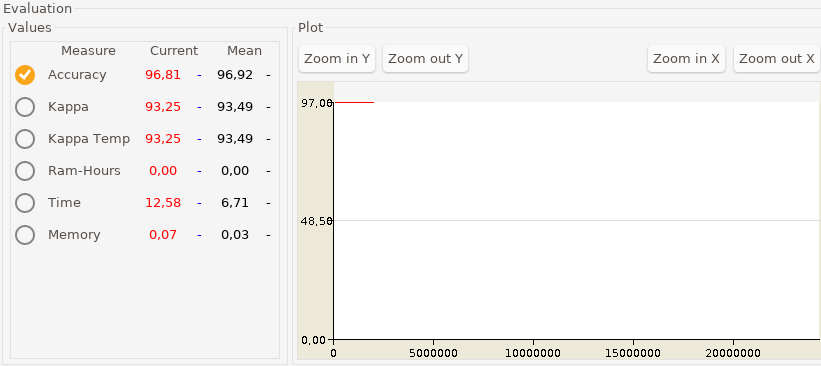
\includegraphics[width=70mm]{imagenes/singledrift_hoffadps3}}
	\caption{Resultados SingleClassifierDrift con semilla 3}
	\label{fig:res53}
\end{figure}

Como se puede ver en las gráficas obtenidas en la GUI de MOA, la precisión
de ambos clasificadores es la misma. A diferencia del ejercicio 2.3,
se utiliza un modelo \textit{SingleClassfierDrift}; por ello, el clasificador se
cambia cuando se detecta un cambio de concepto. Por lo tanto, cada vez que
hay un cambio de concepto se crea un nuevo modelo, tanto para \textit{HoeffdingTree}
como para \textit{HoeffdingAdaptiveTree} y entonces el modelo \textit{HoeffdingAdaptiveTree} se comporta como el modelo \textit{HoeffdingTree} ya que este no detecta el cambio
de concepto. En cambio, en el ejercicio 4 y en el ejercicio 3 sí que hay una diferencia de rendimiento entre ambos clasificadores, ya que el clasificador \textit{HoeffdingAdaptiveTree} puede detectar los cambios de concepto y el otro no. Como similitud en los tres ejercicios está el tipo de flujo que se ha utilizado para comparar el rendimiento de los clasificadores, que siempre ha sido el generado por el generador \textit{RandomRBFGeneratorDrift} con las mismas semillas y parámetros.


\chapter{Parte Teórica}
\section{Preguntas tipo test}
\subsection{Pregunta 1}
El aprendizaje incremental es útil cuando se quiere ganar eficiencia.
\subsection{Pregunta 2}
La minería de flujo de datos se considera cuando el problema genera datos continuamente.
\subsection{Pregunta 3}
La cota Hoeffding sirve para saber cuando hay suficientes datos para una estimación fiable
\subsection{Pregunta 4}
¿Qué características de clústers mantiene el algoritmo BIRCH?
Suma lineal, suma cuadrática y número de objetos.
\subsection{Pregunta 5}
¿El algoritmo Stream maneja el concept drift?
No.
\subsection{Pregunta 6}
¿Qué es el concept drift?
Cambios en la dinámica del problema.
\subsection{Pregunta 7}
¿Cómo gestiona CVFDT el concept drift?
Mantiene árboles alternativos.
\subsection{Pregunta 8}
¿Por qué es útil el ensemble learning en concept drift?
Porque aprovecha la diversidad que se genera en los cambios.
\subsection{Pregunta 9}
¿Cuál es más eficiente entre DDM y ADWIN?
Los dos son muy ineficientes.
\subsection{Pregunta 10}
¿Por qué es controvertida la clasificación en flujo de datos? 
Porque se requiere al oráculo por siempre.

\subsection{Pregunta 11}
¿Cómo gestiona ClueStream el concept drift? 
Mantiene información sobre el tiempo.

\subsection{Pregunta 12}
¿Por qué es complejo generar reglas de asociación en flujo de datos?
Porque para calcular la confianza se requieren muchos datos.
\section{Clasificación y experimentos}
El problema que de clasificación dentro de la minería de flujo de datos trata de predecir la clase de unos datos que van llegando cada cierto tiempo y los algoritmos tratan de maximizar la precisión en la predicción de dichas clases. Para el ejemplo de esta práctica, el objetivo es también maximizar la precisión en la predicción de datos generados con diferentes generadores de flujo de datos, algunos con cambios de concepto, y analizar el comportamiento de dos clasificadores.\newline

Los clasificadores utilizados en la práctica son \textit{HoeffingTree} y \textit{HoeffdingTree adaptativo}, el segundo es la versión adaptada a cambios de concepto del primero.\newline

El clasificador \textit{HoeffdingTree} es un tipo de árbol de decisión utilizados en aprendizaje incremental; estos modelos utilizan la desigualdad de Hoeffding para realizar las particiones del árbol, con esta medida se puede estimar si la media de una variable aleatoria no ha cambiado después de \textit{n} instantes de tiempo; esto es interesante para problemas incrementales ya que el árbol realiza particiones para variable que no han cambiado durante el tiempo, por lo cual la partición que hace sobre dicha variable es fiable. Lo malo de este tipo de algoritmos es que puede necesitar muchos datos para poder realizar una partición sobre los datos, además este primer modelo no es capaz de detectar los cambios en la dinámica de los datos, por lo cual no es apto para problemas donde haya cambios de concepto (la gran mayoría en la realidad).

El clasificador \textit{HoeffdingTree adaptativo} es la versión de \textit{HoeffdingTree} capaz de identificar cambios de concepto. Este algoritmo guarda diferentes versiones del árbol, una vez se produce un cambio de concepto y el árbol actual deja de ser preciso en las predicciones, el algoritmo reemplaza los nodos necesarios para que el árbol se adapte a los nuevos datos. Para el caso de la práctica, el árbol utiliza el algoritmo \textit{ADWIN}, este algoritmo utiliza una ventana principal sobre los datos y comprueba si existen dos ventanas suficientemente grandes y diferentes; si dichas ventanas existen, detecta el cambio de concepto en los datos. Una vez este algoritmo a detectado un cambio de concepto, el árbol modifica sus nodos para adaptarse a sus nuevos datos.

Dentro del desarrollo de la práctica se han utilizado tres métodos de evaluación, el primero de ellos es una evaluación estática de los modelos, el segundo mediante la estrategia \textit{interleaved test-then-train} y el tercero mediante la estrategia \textit{prequential}. La estrategia \textit{interleaves test-then-train}
utiliza primero los datos para testear el modelo, tras esto, re-entrena el modelo con los nuevos datos; la estrategia \textit{prequential} utiliza la misma técnica, la diferencia entre estos dos es la forma en la que calculan la precisión de los clasificadores; en el caso de \textit{interleaved test-then-train} utiliza todos los datos con los datos que se ha entrenado, para el caso de \textit{prequential} utiliza una ventana de un tamaño fijo para utilizar solamente esos datos.

\section{Concept Drift}
El \textit{concept drift} es un problema que se produce en los problemas de minería de flujo de datos, el \textit{concept drift} se trata de una variación en la dinámica de los datos; este cambio de dinámica en los datos hace que los algoritmos clásicos tengan problemas en la predicción de datos una vez se produce este \textit{concept drift}. Por ello, se debe crear nuevos modelos que sean capaces de detectar este cambio de concepto y adaptarse de forma rápida a los datos para que sean útiles en problema del mundo real. Este \textit{concept drift} pueden darse de diferentes maneras, pueden ser de forma abrupta, gradual, incremental, etc... El \textit{concept drift} puede deberse a diferentes razones, como por ejemplo ruido en los datos o variaciones en las características que inicialmente no habían sido contempladas por el modelo.

La primera solución al cambio de concepto se basan en algoritmos basados en aprendizaje incremental. Actualmente existen diferentes alternativas para manejar el \textit{concept drift} en la minería de flujo de datos.

El primero de los enfoques es el aprendizaje online, este tipo de aprendizaje entrena continuamente los modelos mientras que van llegando datos, por ejemplo los \textit{HoeffdingTree adaptativo}.

El segundo enfoque es el aprendizaje mediante ventanas; estos algoritmos se basan en que los datos más recientes tienen más importancia que los datos antiguos, para ello existen diferentes metodologías, como por ejemplo utilizar una ventana deslizantes sobre el conjunto de datos total o ponderar los datos según el tiempo de llegada.

Otro enfoque es el aprendizaje mediante modelos ensemble. Este tipo de enfoque es interesante porque el contexto se puede manejarse mediante la diversidad de los modelos que forman el ensemble. Dentro de este enfoque se utilizan variantes que utilizan predicción mediante votación o por ponderación.

La última de los enfoques es utilizar un algoritmo que detecte el \textit{concept drift} y re-entrene el modelo que se está utilizando para realizar la predicción. Uno de los algoritmos que se encarga de esto es el algoritmo \textit{DDM}, este se fija en la precisión del modelo para detectar el \textit{concept drift}, si la precisión baja mucho durante un espacio de tiempo, se detecta el \textit{concept drift}. Otro algoritmo utilizado para la detección del \textit{concept drift} es \textit{ADWIN}, que ya se ha comentado anteriormente. El problema de estos dos algoritmos es que son ineficientes y por lo tanto no sirven para problemas que manejan cantidades grandes de datos. Otro algoritmo para detección de \textit{concept drift} es \textit{HSP}, este es más eficiente que los dos anteriores comentados y no requiere monitorizar el algoritmo de predicción.

Por lo tanto, se puede ver que el \textit{concept drift} es un problema que debe contemplarse en cualquier problema de minería de flujo de datos e implementarse para conseguir ofrecer buenos resultados tanto en clasificación como en cualquier otro problema de análisis de datos.



\end{document}